
In this chapter the application domain will be analyzed.
Where the problem domain, in \cref{ch:ProblemDomain}, focused on; what information the system should process, the application domain focuses on; how the user will use the system in practice.
This analysis will start with a PACT \cite{Benyon} analysis in \cref{sec:PACT}, where the context of the use of the system will be explored, which delves into the people, their activities, contexts and the technologies used.
Afterwards use cases of the system will be explored in \cref{sec:usecases}, followed by functions that need to support these use cases in \cref{sec:functions}.

\section{PACT analysis}\label{sec:PACT}
When developing an interactive system it is important to design it with the users in mind as the system is being developed for a specific purpose and context.
This is also know as human-centred design.
On the other hand is the machine-centred design where the users are seen as vague, disorganized and have to fit the needs of the machine.
To design human-centred, the developers must explore the users who will eventually use the system and for what purposes they are going to utilize it.

To help understand and reflect upon the users and their relation to an interactive system, the framework \textit{PACT} is used.
PACT is an acronym for \textit{People, Activities, Context}, and \textit{Technology}.

Depending on how well developers have implemented a way to convey their conception of a given system, different users will interpret it differently.
Their interpretation, being based on individual understanding and knowledge, regulates the users interactions with the system and thereby determines what it really does.
A model of this concept can be seen in \cref{fig:PACT-SystemImage}.

\begin{figure}[H]
	\centering
	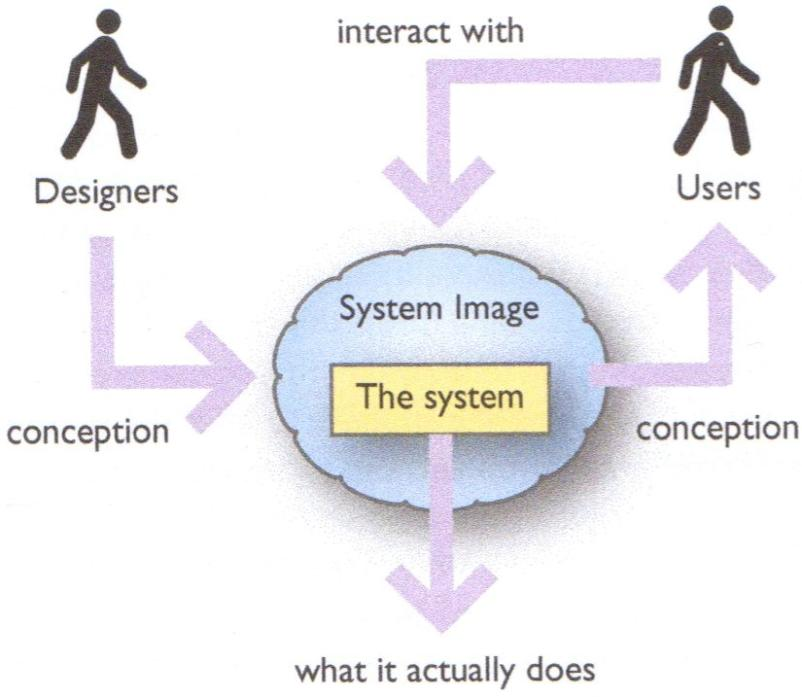
\includegraphics[width=0.5\textwidth]{billeder/SystemImage-Benyon.jpg}
	\caption{\textit{The System Image from \citep[p.~31]{Benyon}}}
	\label{fig:PACT-SystemImage}
\end{figure}

The PACT theory presentation and analysis will be written congruently throughout this section.
First the specific theory will be presented followed by the analysis.

\subsection{People}\label{sec:PACT-people}
People differ from each other in many ways.
This element in the PACT analysis is a way to ponder upon these differences as well as a way to categorize the different users of a system.
Three differences that is, usually, discussed in this part of the analysis are; \textit{physical, psychological}, and \textit{social}.
In this chapter only the physical and social differences will be discussed.

Physical differences covers the relevant ways people differ in physical characteristics.
This could be, differences in perception from the five senses; sight, hearing, touch, smell and taste as well, along with age, height or weight.
An example of a physical difference could be color blindness, which affects about $8\%$ of men and $0.5\%$ of women in the world \cite{ColourBlind}.

Social differences is about how people use a system for different reasons and therefore can have various goals.
Additionally, there is also a big difference in people's expertise levels which affects how an interface might be designed.
This is an important consideration, since designing a system for a homogeneous group of people is  different from designing one for a heterogeneous group. \cite{Benyon}

\subsubsection*{People analysis}
In the case described in this report, see \cref{sec:CaseDescription}, there are four main groups of people that need to be considered.
These are the quality manager, secretary, department heads, and blue-collar workers.
This is a heterogeneous group with IT experience ranging from possibly none to what is required at everyday office work.
Should a blue-collar worker have no IT experience, it seems reasonable to assume that, this blue-collar worker may be cautious of it and the design needs to take this into account.
The group also has different levels of domain expertise ranging from novice to expert, which needs to be considered.
The quality manager is a domain expert and, therefore, has different needs of the system than the blue-collar worker with no expertise.
Furthermore, issues such as colorblindness, and other handicaps, as well as bad memory needs to be considered when designing the system and interface.

\subsection{Activities}\label{sec:PACT-actvities}
It is important to figure out what activities the system needs to support.
First and foremost, the analysis of the activities should focus on the overall \textit{purpose} of the activity.
However, each one of the groups described in \cref{sec:PACT-people} has a different goal in using the system.
The secretary,  quality and department managers need to manage, update and access the handbook, whereas the blue-collar workers only need to access and read certain documents.
This will be further elaborated in \cref{sec:Actors}.
The different kinds of purposes an activity can have is explored below.

\textit{Temporal aspects} covers different features in the system as well as a consideration of how the users' interactions with the system are done during a day.
Starting with the considerations of user interactions, one need to consider among other:

\begin{itemize}
	\item How often is the interactive system used?
	\item Is the interactions with the system done continuously or interrupted?
\end{itemize}

For the temporal aspects in a given system, the developers need to consider things such as; time pressures, peaks and, and the response time of a given activity.

\textit{Cooperation} is the consideration of, whether or not, the activity is done in cooperation with others, alone, or a mix hereof, as well as how and when a possible cooperation is needed.
This is an important consideration, since a system which is done in cooperation with others needs to have an awareness of all the users, be able to coordinate between them and possibly have a communication system implemented as well.
On the other hand, if the activities are done completely alone these features are not necessary.

\textit{Complexity} describes the question of how well-defined the activity is.
Is it a well-defined task which can be done in a simple step-by-step design, or is it a vague task, which would require the users to browse around?

\textit{Safety Critical} has two sides to it.
First is whether or not the activity in itself is ``safety-critical'' where mistakes could be reason for injury or serious accidents.
Second is the consideration of ``what will happen when mistakes and errors are made?'', which is important for any developer to reflect upon.

\textit{The nature of the content} is a more technical reflection of which data requirements are needed for the activity as well as what media it requires.

\subsubsection*{Activities analysis}
In the case of this project, see \cref{sec:CaseDescription}, in terms of temporal aspects during the activities, users may experience interruptions and the system should therefore be simple to use and easy to get back to.

Being easy to use is a feature especially relevant for the blue-collar workers, as they only occasionally need to read documents and therefore are less in contact with the system.
The activities would most often be done during business hours, from 8-16 on weekdays, though may be accessed outside of this time frame as well.

The cooperation aspect is mostly relevant for the  quality manager and department heads, or in more general terms, the administrator and writer roles, as they are maintaining the handbook documents.
Though writing the documents in itself does not require collaboration.
However, after a document has been written, it needs to be approved by other users.
This is one of the most important collaboration aspects in the system.
This sort of communication is partly facilitated by notifications. It is important in the design of these notifications that they are non-obtrusive when the user is focusing on something else. But this is achieved mostly by the notifications only being visible in the browser. Designing the notifications such that they are only dismissed when the task they indicate is complete, turns it into a double feature as a to-do list.
As for the blue-collar worker's activities, there is no cooperation involved, as all they need, is to read the newest, relevant documents individually.

Regarding the complexity; the activities are quite well-defined overall.
The main activities for the administrative personnel is, that whenever a new document has been written, it needs to be approved and then added to the handbook.
Hereby archiving the the old and now outdated document.
The department manager needs to make sure that the affected blue-collar workers read and understand the new documents.

In relation to safety critical aspect, there are no physical safety issues to consider in relation to the system, though there are serious consequences to consider if the documents in the handbook does not live up to regulations, as mentioned in \cref{sec:ISOstandards}.
It is required that the handbook dis up to date and that the elder versions of its documents are stored somewhere.
If this is not upheld the firm could suffer loss of certification, see \cref{sec:standards}, which would result in great loss of revenue.

In terms of the nature of the content, the system should be able to handle Microsoft documents such as Word and Excel as these are the filetypes used to write the documents.
As Ipsen has mentioned, it is also acceptable that the system accepts PDF files instead, as long as she is able to write the document with her preferred text editing software.
Furthermore, the system should support large quantities of these files as the archived versions of the documents would be stored indefinitely.

\subsection{Contexts}
Activities always occur in a context, which will be explored in this section.
Context can be thought of, as something that surrounds activities as well as a feature which binds them together into a whole.
Usually, when considering this point in PACT, the three points: \textit{Physical environment, Social context}, and \textit{Organizational context} are at the main focus.
The analysis will not include the social context as this is not considered relevant for the system development.

The physical environment may cover everything from weather to geographical placement of where the activity is done.
It is an analysis of the surrounding environment which may have effect on how users perform activities.

\subsubsection*{Context analysis}
There are two main physical contexts to consider.
For the quality manager and the secretary, an office context is most likely as they handle administrative work.
For the blue-collar workers, the context could differ dramatically as their functions may differ from each other.
The main focus here, is that the handbook documents should be easily accessible, no matter in which context the blue-collar workers are located.
Previous to this development project, the most common way that the handbooks were used by employees were in a paper format, which allowed the use of the documents in circumstances not conductive to electronic equipment.
It is expected that this practice will continue after the project.

As for the organizational context, there are different factors to consider.
These are Ipsen, who acts as a third party quality manager for a firm in relation to maintaining the handbook.
Then there is the in-house secretary, who Ipsen works the closest with.
There is the CEO, who from time to time reads, writes, and approves the handbook documents.
Lastly, there are the blue-collar workers within the firm whose work and daily tasks vary depending on their positions.

It is because of the structure, of the organization, that there needs to exist different access rights in the system, which are administrator, writer, and reader.
The administrator role is mainly for the quality manager, who is the main person to manage the handbook documents.
There are actors within the firm, the CEO for example, who occasionally needs to write/update documents in the handbook and need writer access rights.
All of the blue-collar workers need to read and understand the specific documents in the handbook, that relates to their work.
These blue-collar workers need reader rights to access the documents.

\subsection{Technologies}
Technologies is the reflection on the medium which interactive system developers work with.
It covers looking into elements such as what medias and technologies are needed to best get input and present the output, and review the communication between the needed devices.
Furthermore, it also examines the content, which concerns the data in the system and its form.
Good content is defined as accurate, up to date, relevant and well presented.

\subsubsection*{Technology analysis}
Since the activities are most often done in an office environment, on a standard PC, the input medias are keyboard and mouse.
In addition, output is presented through a monitor or, for the blue-collar workers on the factory floor, through a printed version of the handbook, or parts of it.
The content displayed to the user, on the monitor, is presented through a web browser.
In \cref{sec:conditions}, it was mentioned that the majority of the users have limited IT-experience.
It is therefore important that the content displayed is simple enough to allow the users to easily navigate and use the system.

Furthermore, the user-to-user communication is usually done through telephone or emails, while it between devices is done over a network, such as the internet.
Lastly, the system-to-user communication is done through notifications.
These will be sent every time a document, relevant to the user, has been updated and the user therefore has to read it, or when the user has been assigned to approve a new version.

